\addcontentsline{toc}{chapter}{Habakkuk}

% Safely inserts your illustration full-bleed on its own page.
% This completely bypasses the page builder, headers, and geometry bugs!
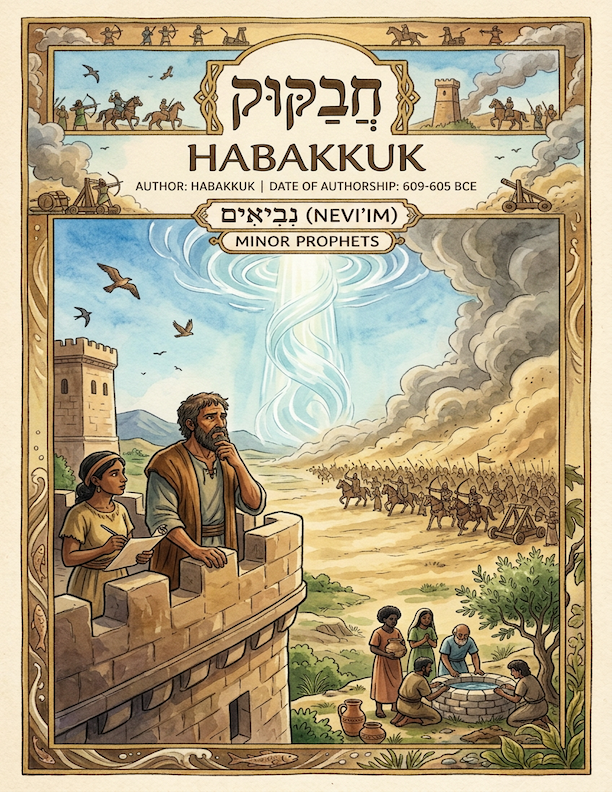
\includepdf[pages=1, fitpaper=false, width=\paperwidth, height=\paperheight, keepaspectratio=false]{images/divider2/habakkuk_2.png} 
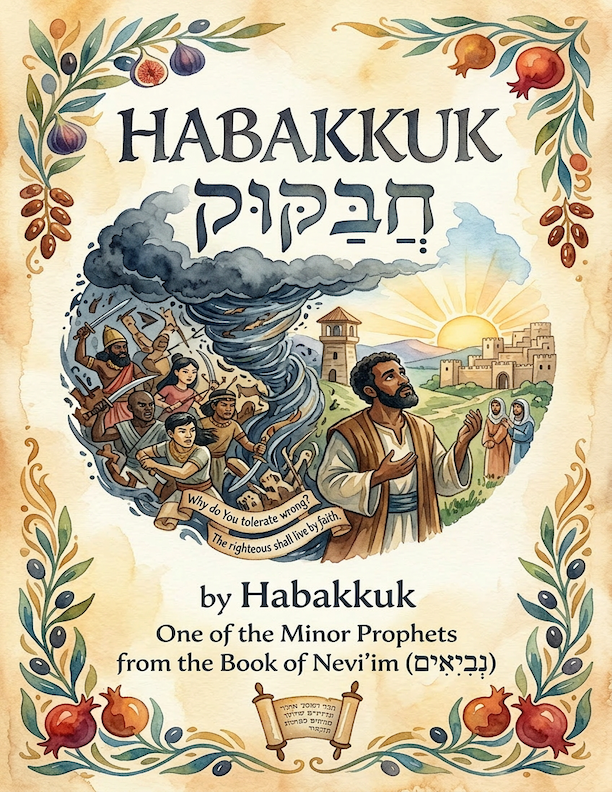
\includepdf[pages=1, fitpaper=false, width=\paperwidth, height=\paperheight, keepaspectratio=false]{images/divider1/habakkuk.png}

\includepdf[pages=1, fitpaper=false, width=\paperwidth, height=\paperheight, , keepaspectratio=false]{images/8.5x11-Dot-Grid.png}

\includepdf[pages=1, fitpaper=false, width=\paperwidth, height=\paperheight, , keepaspectratio=false]{images/8.5x11-Dot-Grid.png}
\mybook{Habakkuk}
\vspace{-1.36in}

\mychapter{} \myverse*{}The revelation which Habakkuk the prophet saw. \myverse{}LORD,\footnote{1:2 When rendered in ALL CAPITAL LETTERS, “LORD” or “GOD” is the translation of God’s Proper Name.} how long will I cry, and you will not hear? I cry out to you “Violence!” and will you not save? \myverse{}Why do you show me iniquity, and look at perversity? For destruction and violence are before me. There is strife, and contention rises up. \myverse{}Therefore the law is paralyzed, and justice never prevails; for the wicked surround the righteous; therefore justice comes out perverted.


\myverse{}“Look among the nations, watch, and wonder marvelously; for I am working a work in your days which you will not believe though it is told you. \myverse{}For, behold,\footnote{1:6 “Behold”, from “הִנֵּה”, means look at, take notice, observe, see, or gaze at. It is often used as an interjection.} I am raising up the Kasdim, that bitter and hasty nation who march through the width of the earth, to possess dwelling places that are not theirs. \myverse{}They are feared and dreaded. Their judgment and their dignity proceed from themselves. \myverse{}Their horses also are swifter than leopards, and are more fierce than the evening wolves. Their horsemen press proudly on. Yes, their horsemen come from afar. They fly as an eagle that hurries to devour. \myverse{}All of them come for violence. Their hordes face forward. They gather prisoners like sand. \myverse{}Yes, they scoff at kings, and princes are a derision to them. They laugh at every stronghold, for they build up an earthen ramp and take it. \myverse{}Then they sweep by like the wind and go on. They are indeed guilty, whose strength is their god.”


\myverse{}Aren’t you from everlasting, LORD my God,\footnote{1:12 The Hebrew word rendered “God” is “אֱלֹהִ֑ים” (Elohim).} my Holy One? We will not die. LORD, you have appointed them for judgment. You, Rock, have established him to punish. \myverse{}You who have purer eyes than to see evil, and who cannot look on perversity, why do you tolerate those who deal treacherously and keep silent when the wicked swallows up the man who is more righteous than he, \myverse{}and make men like the fish of the sea, like the creeping things that have no ruler over them? \myverse{}He takes up all of them with the hook. He catches them in his net and gathers them in his dragnet. Therefore he rejoices and is glad. \myverse{}Therefore he sacrifices to his net and burns incense to his dragnet, because by them his life is luxurious and his food is good. \myverse{}Will he therefore continually empty his net, and kill the nations without mercy?


% HABAKKUK 2
\mychapter{} \myverse*{}I will stand at my watch and set myself on the ramparts, and will look out to see what he will say to me, and what I will answer concerning my complaint.


\myverse{}The LORD answered me, “Write the vision, and make it plain on tablets,
that he who runs may read it. \myverse{}For the vision is yet for the appointed time, and it hurries toward the end, and won’t prove false. Though it takes time, wait for it, because it will surely come. It won’t delay. \myverse{}Behold, his soul is puffed up. It is not upright in him, but the righteous will live by his faith. \myverse{}Yes, moreover, wine is treacherous: an arrogant man who doesn’t stay at home, who enlarges his desire as Sheol;\footnote{2:5 Sheol is the place of the dead.} he is like death and can’t be satisfied, but gathers to himself all nations and heaps to himself all peoples.


\myverse{}Won’t all these take up a parable against him, and a taunting proverb against him, and say, ‘Woe to him who increases that which is not his, and who enriches himself by extortion! How long?’ \myverse{}Won’t your debtors rise up suddenly, and wake up those who make you tremble, and you will be their victim? \myverse{}Because you have plundered many nations, all the remnant of the peoples will plunder you because of men’s blood, and for the violence done to the land, to the city and to all who dwell in it.


\myverse{}Woe to him who gets an evil gain for his house, that he may set his nest on high, that he may be delivered from the hand of evil! \myverse{}You have devised shame to your house by cutting off many peoples, and have sinned against your soul. \myverse{}For the stone will cry out of the wall, and the beam out of the woodwork will answer it.


\myverse{}Woe to him who builds a town with blood, and establishes a city
by iniquity! \myverse{}Behold, isn’t it from the LORD of Hosts that the peoples labor for the fire, and the nations weary themselves for vanity? \myverse{}For the earth will be filled with the knowledge of the LORD’s glory, as the waters cover the sea.


\myverse{}“Woe to him who gives his neighbor drink, pouring your inflaming wine until they are drunk, so that you may gaze at their naked bodies! \myverse{}You are filled with shame, and not glory. You will also drink and be exposed! The cup of the LORD’s right hand will come around to you, and disgrace will cover your glory. \myverse{}For the violence done to Lebanon will overwhelm you, and the destruction of the animals will terrify you, because of men’s blood and for the violence done to the land, to every city and to those who dwell in them.


\myverse{}“What value does the engraved image have, that its maker has engraved it; the molten image, even the teacher of lies, that he who fashions its form trusts in it, to make mute idols? \myverse{}Woe to him who says to the wood, ‘Awake!’ or to the mute stone, ‘Arise!’ Shall this teach? Behold, it is overlaid with gold and silver, and there is no breath at all within it. \myverse{}But the LORD is in his holy temple. Let all the earth be silent before him!”


% HABAKKUK 3
\mychapter{} \myverse*{}A prayer of Habakkuk, the prophet, set to victorious music.


\myverse{}LORD, I have heard of your fame.

I stand in awe of your deeds, LORD.

Renew your work in the middle of the years.

In the middle of the years make it known.

In wrath, you remember mercy.


\myverse{}God came from Teman,

the Holy One from Mount Paran.

\rightline{Selah.}
\vspace{\baselineskip} 

His glory covered the heavens,

and his praise filled the earth.


\myverse{}His splendor is like the sunrise.

Rays shine from his hand, where his power is hidden.


\myverse{}Plague went before him,

and pestilence followed his feet.


\myverse{}He stood, and shook the earth.

He looked, and made the nations tremble.

The ancient mountains were crumbled.

The age-old hills collapsed.

His ways are eternal.


\myverse{}I saw the tents of Cushan in affliction.

The dwellings of the land of Midian trembled.


\myverse{}Was the LORD displeased with the rivers?

Was your anger against the rivers,

or your wrath against the sea,

that you rode on your horses,

on your chariots of salvation?


\myverse{}You uncovered your bow.

You called for your sworn arrows.

\rightline{Selah.}
\vspace{\baselineskip}

You split the earth with rivers.


\myverse{}The mountains saw you, and were afraid.

The storm of waters passed by.

The deep roared and lifted up its hands on high.


\myverse{}The sun and moon stood still in the sky

at the light of your arrows as they went,

at the shining of your glittering spear.


\myverse{}You marched through the land in wrath.

You threshed the nations in anger.


\myverse{}You went out for the salvation of your people,

for the salvation of your anointed.

You crushed the head of the land of wickedness.

You stripped them head to foot.

\rightline{Selah.}
\vspace{\baselineskip} 

\myverse{}You pierced the heads of his warriors with their own spears.

They came as a whirlwind to scatter me,

gloating as if to devour the wretched in secret.


\myverse{}You trampled the sea with your horses,

churning mighty waters.


\myverse{}I heard, and my body trembled.

My lips quivered at the voice.

Rottenness enters into my bones, and I tremble in my place

because I must wait quietly for the day of trouble,

for the coming up of the people who invade us.


\myverse{}For even though the fig tree doesn’t flourish,

nor fruit be in the vines,

the labor of the olive fails,

the fields yield no food,

the flocks are cut off from the fold,

and there is no herd in the stalls,


\myverse{}yet I will rejoice in the LORD.

I will be joyful in the God of my salvation!


\myverse{}GOD, the Lord,\footnote{3:19 The word translated “Lord” (mixed case) is “Adonai.”} is my strength.

He makes my feet like deer’s feet,

and enables me to go in high places.

For the music director, on my stringed instruments.


